% See section 11 of the User Manual for version history
%
%%%%%%%%%%%%%%%%%%%%%%%%%%%%%%%%%%%%%%%%%%%%%%%%%%%%%%%%%%%%%%%%%%%%%%
%%                                                                 %%
%% Please do not use \input{...} to include other tex files.       %%
%% Submit your LaTeX manuscript as one .tex document.              %%
%%                                                                 %%
%% All additional figures and files should be attached             %%
%% separately and not embedded in the \TeX\ document itself.       %%
%%                                                                 %%
%%%%%%%%%%%%%%%%%%%%%%%%%%%%%%%%%%%%%%%%%%%%%%%%%%%%%%%%%%%%%%%%%%%%%

%%\documentclass[referee,sn-basic]{sn-jnl}% referee option is meant for double line spacing

%%=======================================================%%
%% to print line numbers in the margin use lineno option %%
%%=======================================================%%

%%\documentclass[lineno,pdflatex,sn-basic]{sn-jnl}% Basic Springer Nature Reference Style/Chemistry Reference Style

%%=========================================================================================%%
%% the documentclass is set to pdflatex as default. You can delete it if not appropriate.  %%
%%=========================================================================================%%

%%\documentclass[sn-basic]{sn-jnl}% Basic Springer Nature Reference Style/Chemistry Reference Style

%%Note: the following reference styles support Namedate and Numbered referencing. By default the style follows the most common style. To switch between the options you can add or remove “Numbered” in the optional parenthesis. 
%%The option is available for: sn-basic.bst, sn-chicago.bst%  
 
%%\documentclass[pdflatex,sn-nature]{sn-jnl}% Style for submissions to Nature Portfolio journals
%%\documentclass[pdflatex,sn-basic]{sn-jnl}% Basic Springer Nature Reference Style/Chemistry Reference Style
\documentclass[sn-mathphys-num]{sn-jnl}% Math and Physical Sciences Numbered Reference Style
%%\documentclass[pdflatex,sn-mathphys-ay]{sn-jnl}% Math and Physical Sciences Author Year Reference Style
%%\documentclass[pdflatex,sn-aps]{sn-jnl}% American Physical Society (APS) Reference Style
%%\documentclass[pdflatex,sn-vancouver-num]{sn-jnl}% Vancouver Numbered Reference Style
%%\documentclass[pdflatex,sn-vancouver-ay]{sn-jnl}% Vancouver Author Year Reference Style
%%\documentclass[pdflatex,sn-apa]{sn-jnl}% APA Reference Style
%%\documentclass[pdflatex,sn-chicago]{sn-jnl}% Chicago-based Humanities Reference Style

%%%% Standard Packages
%%<additional latex packages if required can be included here>

\usepackage{graphicx}%
\usepackage{amsmath,amssymb,amsfonts}%
\usepackage{amsthm}%
\usepackage[title]{appendix}%
\usepackage{xcolor}%
\usepackage{textcomp}%
\usepackage{booktabs}%
\usepackage{enumitem}%
%%%%

%%%%%=============================================================================%%%%
%%%%  Remarks: This template is provided to aid authors with the preparation
%%%%  of original research articles intended for submission to journals published 
%%%%  by Springer Nature. The guidance has been prepared in partnership with 
%%%%  production teams to conform to Springer Nature technical requirements. 
%%%%  Editorial and presentation requirements differ among journal portfolios and 
%%%%  research disciplines. You may find sections in this template are irrelevant 
%%%%  to your work and are empowered to omit any such section if allowed by the 
%%%%  journal you intend to submit to. The submission guidelines and policies 
%%%%  of the journal take precedence. A detailed User Manual is available in the 
%%%%  template package for technical guidance.
%%%%%=============================================================================%%%%

%% as per the requirement new theorem styles can be included as shown below
% \theoremstyle{thmstyleone}%
\newtheorem{theorem}{Theorem}%  meant for continuous numbers
%%\newtheorem{theorem}{Theorem}[section]% meant for sectionwise numbers
%% optional argument [theorem] produces theorem numbering sequence instead of independent numbers for Proposition
\newtheorem{proposition}[theorem]{Proposition}% 
\newtheorem{lemma}[theorem]{Lemma}%
\newtheorem{corollary}[theorem]{Corollary}%

% 定义定义、示例类环境（通常使用正体）
\newtheorem{definition}[theorem]{Definition}%
\newtheorem{example}[theorem]{Example}%
\newtheorem{remark}[theorem]{Remark}%

\raggedbottom
%%\unnumbered% uncomment this for unnumbered level heads

\begin{document}

\title[Article Title]{Superellipsoid-Constrained Bidirectional RRT: Path Planning with Adaptive Asymmetric Dual-Super-Ellipsoidal Constrained Sampling}

\author[1]{\fnm{Yan} \sur{Wu}}\email{Wuyan613613@126.com}
\author*[1]{\fnm{Xingyu} \sur{Guo}}\email{gxyhaoxianghenlihai@gmail.com}
\author[1]{\fnm{Muchun} \sur{Fan}}\email{13663358065@163.com}
\author[1]{\fnm{Feng} \sur{Hong}}\email{19512246233@163.com}
\author[1]{\fnm{Hongyu} \sur{Gao}}\email{2014922529@qq.com}
\author[1]{\fnm{Jianyu} \sur{Zheng}}\email{15156139538@163.com}


\affil[1]{\orgdiv{School of Mechanical Engineering}, \orgname{Shanghai Institute of Technology}, \orgaddress{\street{No. 100 Haiquan Road}, \city{Shanghai}, \postcode{201418}, \state{Shanghai}, \country{China}}}

%%==================================%%
%% Sample for unstructured abstract %%
%%==================================%%

\abstract{Sampling-based path planning algorithms commonly suffer from excessive invalid samples, slow convergence, and reduced success rates in high-obstacle-density environments. This paper presents SC-RRT, a path planning algorithm based on adaptive asymmetric dual-super-ellipsoid constrained sampling. Within a bidirectional parallel expansion framework, SC-RRT employs an intermediate meeting point $\mathbf{x}_{\text{meet}}$ to decompose the global task into staged subproblems. Scale-variable, asymmetric informed sampling subsets are constructed in both directions to concentrate sampling toward feasible regions with greater improvement potential, forming the Adaptive Dual-Super-Ellipsoid Constrained Sampling strategy (ADCS). To suppress invalid sampling caused by over-inflation or premature contraction of the informed subset due to cost estimation bias, a Search State Feedback Online Regulation mechanism (SSFOR) is developed. SSFOR uses the historical evolution of the optimal path cost to perform closed-loop adjustment of the super-ellipsoid expansion factor $\gamma$ and heuristic sampling probability $p$, enabling the informed subset to evolve with search progress while reducing redundant expansion. Asymmetric super-ellipsoidal constraints further sharpen resolution along feasible passage directions. Simulation experiments show that SC-RRT reduces path length by approximately 10.5\% compared with Dynamic-RRT, achieving a path efficiency of 0.9553. Although path quality is marginally lower than Informed RRT*, planning time is only 16.2\% of the latter with node count reduced by 94.2\%. SC-RRT thus balances path quality, planning efficiency, and computational cost without prior parameter tuning; its modular ADCS and SSFOR components can be independently integrated into other RRT-based frameworks.}

%%================================%%
%% Sample for structured abstract %%
%%================================%%

% \abstract{\textbf{Purpose:} The abstract serves both as a general introduction to the topic and as a brief, non-technical summary of the main results and their implications. The abstract must not include subheadings (unless expressly permitted in the journal's Instructions to Authors), equations or citations. As a guide the abstract should not exceed 200 words. Most journals do not set a hard limit however authors are advised to check the author instructions for the journal they are submitting to.
% 
% \textbf{Methods:} The abstract serves both as a general introduction to the topic and as a brief, non-technical summary of the main results and their implications. The abstract must not include subheadings (unless expressly permitted in the journal's Instructions to Authors), equations or citations. As a guide the abstract should not exceed 200 words. Most journals do not set a hard limit however authors are advised to check the author instructions for the journal they are submitting to.
% 
% \textbf{Results:} The abstract serves both as a general introduction to the topic and as a brief, non-technical summary of the main results and their implications. The abstract must not include subheadings (unless expressly permitted in the journal's Instructions to Authors), equations or citations. As a guide the abstract should not exceed 200 words. Most journals do not set a hard limit however authors are advised to check the author instructions for the journal they are submitting to.
% 
% \textbf{Conclusion:} The abstract serves both as a general introduction to the topic and as a brief, non-technical summary of the main results and their implications. The abstract must not include subheadings (unless expressly permitted in the journal's Instructions to Authors), equations or citations. As a guide the abstract should not exceed 200 words. Most journals do not set a hard limit however authors are advised to check the author instructions for the journal they are submitting to.}

\keywords{Sampling-based path planning, Informed sampling, bidirectional tree search, online parameter regulation, motion planning}

%%\pacs[JEL Classification]{D8, H51}

%%\pacs[MSC Classification]{35A01, 65L10, 65L12, 65L20, 65L70}

\maketitle

\section{Introduction}\label{sec1}

With the rapid advancement of Industry 4.0 and service robotics, intelligent robots have become a key driver of automation and operational efficiency across manufacturing, service, and related sectors~\cite{zhong2017intelligent,wirtz2018brave,mac2016heuristic}. Their application scope has expanded from structured factory settings to dynamic, complex environments where humans and robots work in close collaboration~\cite{ajoudani2018progress,villani2018survey}. Accordingly, in-depth research into robot path planning algorithms for complex environments carries not only considerable theoretical value, but also practical significance for advancing the real-world engineering deployment of intelligent robots. The core objective of path planning is to generate a collision-free trajectory for a robot within a known configuration space defined by a start point and a goal point, subject to kinematic constraints, while balancing two fundamental requirements: real-time responsiveness and path optimality~\cite{lavalle2006planning,latombe2012robot}. In dynamic environments, randomly distributed obstacles and system uncertainties further compound the difficulty of planning. The shrinkage of the feasible region under sampling constraints and the resulting decline in tree growth efficiency are particularly pronounced~\cite{kingston2018sampling}, making the simultaneous achievement of fast convergence and high-quality paths a central challenge in current research~\cite{mohanan2018survey, aggarwal2020path}.

The Rapidly Exploring Random Tree (RRT) algorithm and its bidirectional variants, such as Bidirectional RRT*, are classical sampling-based path planning methods~\cite{elbanhawi2014sampling,karaman2011sampling}. Owing to their probabilistic completeness and ease of implementation, they have been widely applied in complex environments~\cite{lavalle1998rapidly, lavalle2001randomized}. However, the traditional Bidirectional RRT* algorithm still suffers from inherent limitations, such as strong randomness in the sampling process, low search efficiency, and insufficient geometric smoothness of the planned paths~\cite{kuffner2000rrt,gammell2021asymptotically}. These limitations restrict its performance in scenarios involving large-scale environments, dense obstacles, or dynamically distributed obstacles~\cite{qureshi2015intelligent,ding2023improved}. Researchers have proposed various improvement strategies from the perspectives of sampling guidance, coordination of search strategies, and path structure optimization. A representative line of work enhances convergence efficiency by improving the bidirectional search framework and sampling guidance mechanisms, with particular emphasis on improving accessibility in difficult-to-sample scenarios such as narrow passages~\cite{noreen2016optimal}. ARRT-Connect~\cite{li2021adaptive}, proposed by Li and Chen (2022), as well as ABQ-RRT*~\cite{huang2024adaptive} based on similar principles, adaptively adjust the sampling strategy according to the scale of unexplored regions identified through dual-tree exploration. By incorporating the principal component analysis (PCA) approach introduced by Tahirovic and Ferizbegovic (2018) in RRT~\cite{tahirovic2018rapidly}, these methods enhance the directional growth of trees within elongated feasible corridors, thereby accelerating exploration and connectivity in narrow environments.

However, such methods may still generate a large number of redundant sampling points in regions unrelated to the optimal path when operating in high-dimensional spaces or complex environments with multiple passages, thereby reducing overall planning efficiency. In particular, as the environment scale increases or obstacle density rises, fixed sampling bias strategies struggle to adapt to the varying demands of different search stages, leading to diminished guidance effectiveness of the informed subset. Informed RRT* proposed by Gammell et al.~\cite{gammell2014informed,gammell2018informed} restricts the sampling space to an informed subset defined by a super-ellipsoid with the start and goal states as its foci, thereby concentrating the sampling process on regions that can potentially improve the cost of the current best path. This work establishes the theoretical foundation for cost-guided constrained sampling. Building upon this foundation, Gammell et al. further proposed the BIT* algorithm~\cite{gammell2015batch,gammell2020batch}, which unifies informed sampling and graph search into a heuristic search over an implicit random geometric graph, thereby further improving planning efficiency in high-dimensional scenarios. To further reduce the sensitivity of fixed super-ellipsoids to cost estimation bias, recent studies have attempted to introduce dynamic corridor constraints~\cite{yuan2023improved} or adaptive bidirectional super-ellipsoid sampling~\cite{zeng2025abf} to enhance the adaptability of the sampling domain. The Dynamic-RRT algorithm proposed by Zhao et al. innovatively introduces a heuristic super-ellipsoid constrained sampling mechanism. By estimating the path cost through expanded nodes, it restricts the sampling space to a super-ellipsoid with the start and goal states as its foci and the estimated path length as the major axis, thereby significantly improving the effectiveness of new node generation~\cite{zhao2023dynamic}. Meanwhile, the algorithm incorporates the Pareto Dominance principle~\cite{deb2002fast} and dynamic programming concepts. By selecting Pareto-optimal nodes as new starting points to decompose the planning problem, it further reduces convergence time while ensuring path length optimization. Its performance is significantly superior to classical algorithms such as RRT, RRT*, and Informed RRT. Such methods effectively balance convergence speed and path quality through sampling space constraints and problem decomposition strategies. However, the performance of the sampling constraint mechanism in this algorithm still heavily depends on the accuracy of path cost estimation. When the cost is overestimated, the ellipsoidal constraint region becomes excessively large, leading to a considerable number of invalid samples; when the cost is underestimated, the constraint region shrinks prematurely, potentially excluding feasible optimal paths from the sampling space and causing the algorithm to converge to a suboptimal solution or even fail. Moreover, Dynamic-RRT adopts a unidirectional search framework, in which the informed subset is defined solely by the start and goal as focal points. In complex environments, its ability to guide the global search direction remains limited, and redundant expansions may still occur.

Overall, existing improvement methods still exhibit a pronounced trade-off between efficiency and optimality. While sampling guidance or bidirectional connectivity strategies can accelerate the acquisition of feasible solutions, they generally lack guarantees of asymptotic optimality. In contrast, cost-driven constrained sampling and problem decomposition approaches can increase the proportion of effective samples and improve path quality; however, their performance is highly sensitive to the accuracy of cost estimation. Moreover, the constraint domains are typically static or only weakly adaptive, which may lead to excessive shrinkage in the early search stage, reducing reachability, or cause oscillations in sampling ratios and tree expansion behavior when cost values fluctuate, thereby weakening global robustness and convergence consistency.

To this end, this paper proposes an SC-RRT algorithm based on an adaptive asymmetric dual-super-ellipsoid constrained sampling subset. Within a bidirectional parallel search framework guided by intermediate points, the algorithm constructs asymmetric dual-super-ellipsoid sampling subsets on the start and goal sides that can independently expand and contract. To overcome the sensitivity of traditional constrained sampling to cost estimation bias and to prevent premature shrinkage or ineffective expansion of the sampling space, a search state feedback-based online regulation mechanism is established. Using the current best path cost and its historical evolution as feedback, a closed-loop control strategy is employed to adjust the scale of the super-ellipsoid informed subsets. During the stage when a stable feasible solution has not yet been obtained, the constraints are moderately relaxed to enhance exploration coverage; once feasible paths emerge and continue to improve, the constraints are progressively strengthened to increase effective sampling density and suppress redundant expansions. In this way, a controllable dynamic balance is achieved among convergence speed, path quality, and search stability. Comparative experiments are conducted in representative scenarios with varying obstacle densities and spatial dimensions, using Dynamic-RRT and classical RRT variants as baselines. The effectiveness of the proposed mechanisms is systematically evaluated in terms of path length, planning time, node scale, and path smoothness. 

\section{Proposed Method}\label{sec2}



To establish the mathematical model of the path planning problem~\cite{choset2005principles}, the Cartesian workspace $ W \subseteq \mathbb{R}^m $ and the configuration space $ C \subseteq \mathbb{R}^n $ are defined, where m and n denote the corresponding dimensions, respectively~\cite{lynch2017modern}. Let the state be defined as:
\[
\mathbf{x} \in W
\]
and partition the space into:
\begin{itemize}
    \item Collision-free region: $ W_{\text{free}} $ (white area)
    \item Obstacle region: $ W_{\text{obs}} $ (black circular obstacles)
\end{itemize}
such that:
\[
W = W_{\text{free}} \cup W_{\text{obs}}
\]

The planning start and goal states are denoted by $\mathbf{x}_{\text{start}}$ and $\mathbf{x}_{\text{goal}}$, respectively, where both satisfy $\mathbf{x}_{\text{start}}, \mathbf{x}_{\text{goal}} \in W_{\text{free}}$, as illustrated in Figure~\ref{fig:sc_rrt_overview}.


The SC-RRT algorithm constructs two random trees $T_A$ and $T_B$ from the start state $\mathbf{x}_{\text{start}}$ and the goal state $\mathbf{x}_{\text{goal}}$, respectively, and introduces a dynamic intermediate point $\mathbf{x}_{\text{meet}}$, thereby decoupling the global search into two subproblems: ``start--intermediate'' and ``goal--intermediate,'' as defined in Equation~\eqref{eq:superellipsoid}. The intermediate point $\mathbf{x}_{\text{meet}}$ is updated online based on the bidirectional search states. Unlike a traditional single static ellipsoid, the super-ellipsoid constructed in this paper does not maintain a fixed shape. Its parameters are dynamically updated as the path cost improves and the intermediate point shifts. Using $\mathbf{x}_{\text{meet}}$ as a bridge, the super-ellipsoid adaptively expands and contracts according to changes in path cost and the exploration states during the search process. Sampling constraints are constructed separately on the start side and the goal side, ensuring coverage of potentially optimal paths while progressively tightening the sampling domain boundaries, thereby effectively reducing invalid samples.

\begin{figure}[h]
    \centering
    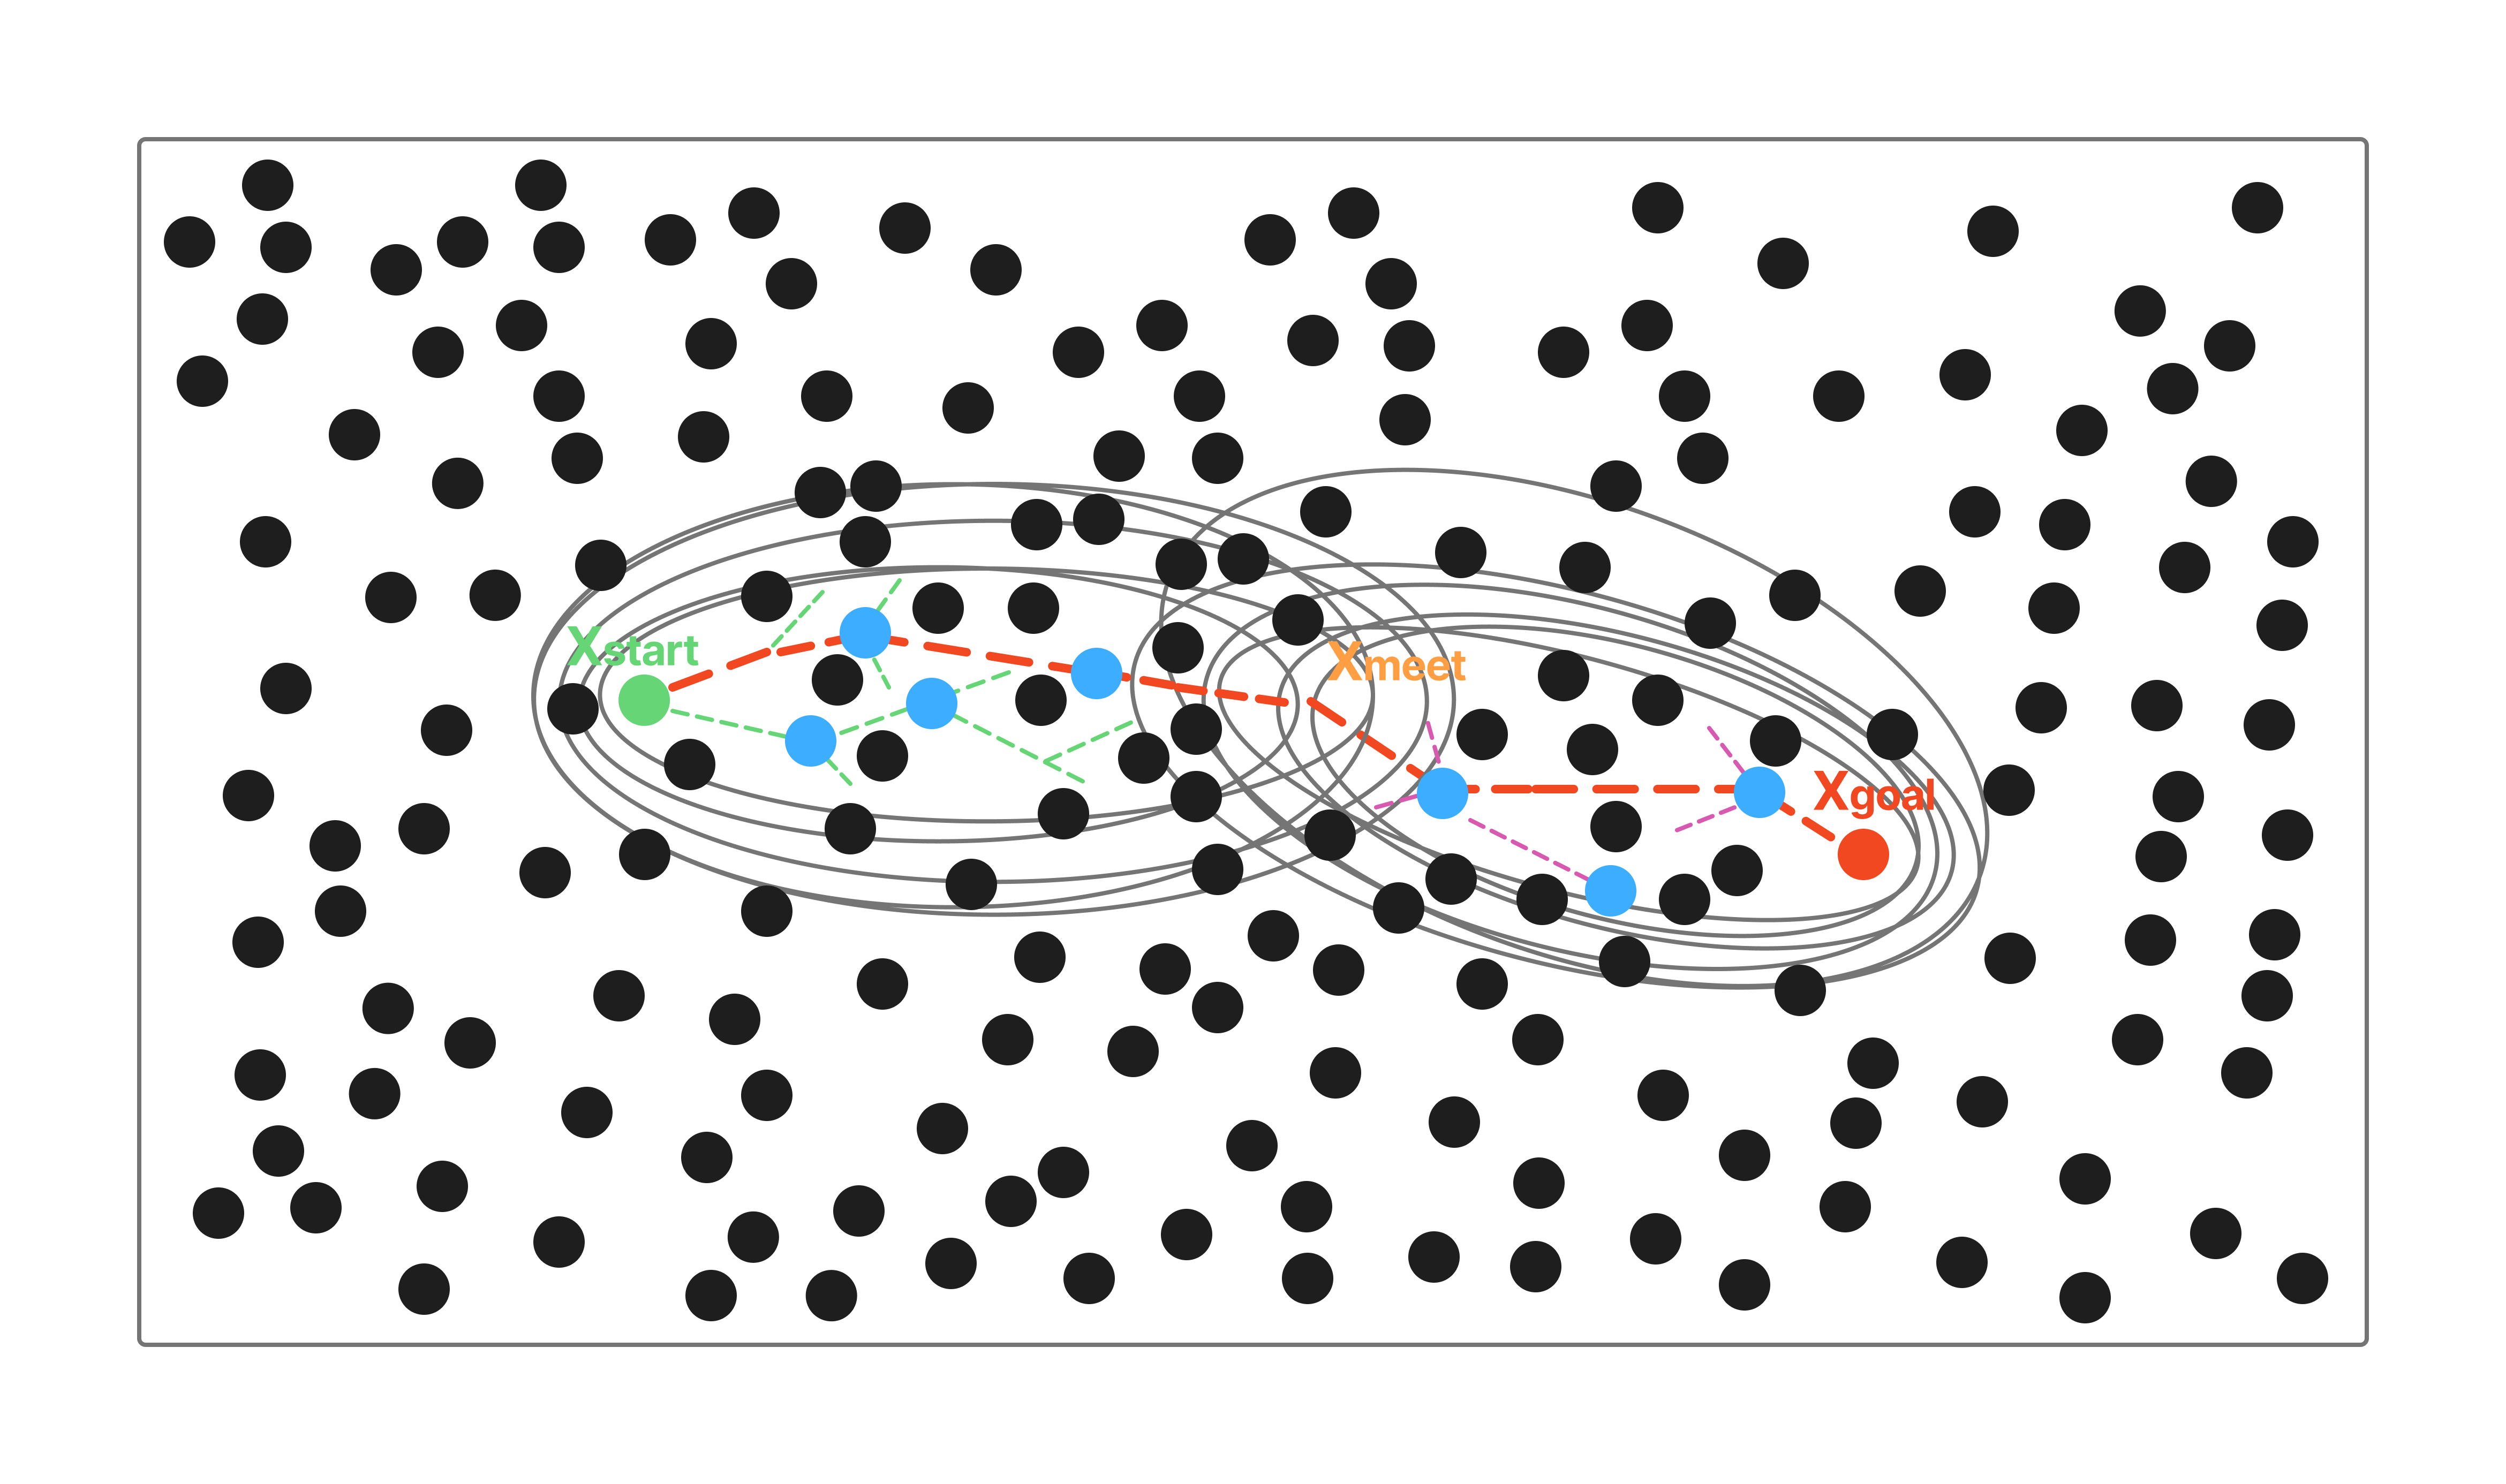
\includegraphics[width=0.8\textwidth]{fig1.png} 
    \caption{Schematic Diagram of the Search State-Driven Adaptive Asymmetric dual-super-ellipsoid Constrained Sampling SC-RRT Path Planning Algorithm}
    \label{fig:sc_rrt_overview}
\end{figure}


\subsection{An Adaptive Asymmetric Dual-Super-Ellipsoid Constrained Sampling (ADCS) Strategy}\label{subsec2}

This paper proposes an asymmetric dual-super-ellipsoidal constrained sampling subset mechanism, as illustrated in Figure~\ref{fig:adcs_flowchart}, to achieve asymmetric regulation of the sampling domain. Unlike the Probabilistic Roadmap (PRM) method~\cite{kavraki2002probabilistic}, which adopts an offline planning paradigm based on a multi-query graph structure, the proposed approach balances global exploration and local refined search during bidirectional tree expansion. Ultimately, it achieves simultaneous reductions in path length, planning time, and the number of nodes. 



The core of this sampling strategy lies in dynamically computing the constraint parameters of the super-ellipsoid. For either direction, taking the start side as an example, it is defined as follows: 

\begin{equation}
    \label{eq:superellipsoid}
    S_j(x) = \left\{ x \in \mathbb{R}^n \;\middle|\; \|x - f_1\| + \|x - f_2\| \leq \gamma \cdot C_{\text{best}}^A, \; s(c_s) \right\}
\end{equation}

\noindent where:
\begin{itemize}[leftmargin=*, label=\textbullet]
    \item $\gamma$ denotes the expansion coefficient adaptively adjusted online by the SSFOR mechanism;
    \item $C_{\text{best}}^A$ denotes the estimated optimal total cost from the start side based on heuristic evaluation;
    \item $\|\mathbf{x} - \mathbf{f}_1\|$ denotes the accumulated path cost from the start node $\mathbf{x}_{\text{start}}$ to node $\mathbf{x}$;
    \item $\|\mathbf{x} - \mathbf{f}_2\|$ denotes the heuristic distance from node $\mathbf{x}$ to the intermediate point $\mathbf{x}_{\text{meet}}$.
\end{itemize}

\begin{figure}[h]
    \centering
    % 确保路径和文件名与左侧文件树完全一致
    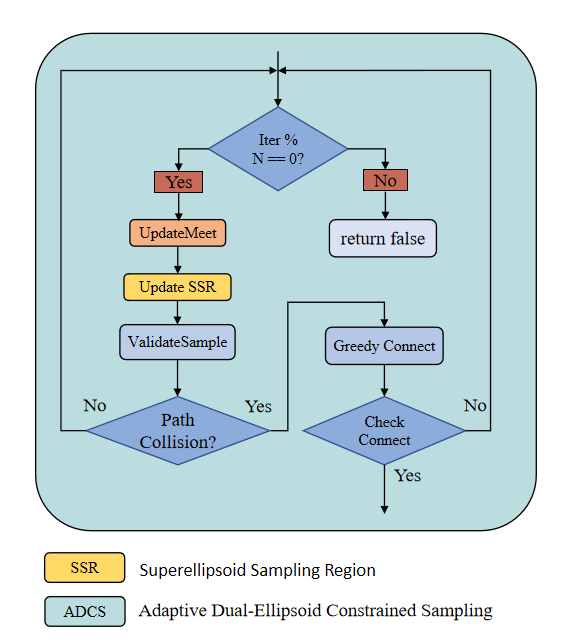
\includegraphics[width=0.8\textwidth]{fig2ADCS.png} 
    \caption{Flowchart of the Adaptive Asymmetric dual-super-ellipsoid Constrained Sampling Strategy}
    \label{fig:adcs_flowchart}
\end{figure}


The goal-side super-ellipsoid is defined analogously. The two super-ellipsoids are updated independently, forming an asymmetric constraint structure. In each iteration, informed sampling is conducted within the above super-ellipsoids with probability $p$; with a certain probability, biased sampling is performed toward the optimal node selected from the opposite tree according to the Pareto dominance principle; and with the remaining probability, global uniform sampling is carried out. This ensures that the search remains focused on effective regions while preserving global coverage capability.



For each newly expanded node, a direct connection to the opposite tree is attempted first. If the distance exceeds the threshold, the opposite tree greedily advances toward it. Once the two trees are successfully connected, node rewiring optimization and adaptive smoothing are performed on the concatenated path~\cite{ravankar2018path,yang2010analytical}, yielding the final feasible path.



\subsection{Search State Feedback-Based Online Regulation (SSFOR) Mechanism}\label{subsec3}

The effectiveness of ADCS depends on the timely adjustment of the expansion coefficient $\gamma$ and the informed sampling ratio $p$. Existing convergence-acceleration methods, such as path-biased sampling~\cite{nasir2013rrt}, batch forward-propagation search~\cite{janson2015fast}, cost lower-bound trade-off strategies~\cite{salzman2016asymptotically}, and anytime planning frameworks~\cite{ferguson2006anytime,karaman2011anytime}, generally adopt preset static parameters. Heuristic sampling pruning methods~\cite{akgun2011sampling} also require predefined thresholds, and thus lack online feedback regulation based on the search state. To address this limitation, this paper proposes the SSFOR mechanism to implement closed-loop regulation of both parameters, as detailed in the flowchart of Figure~\ref{fig:ssfor_flowchart}. The relative rate of decrease in the estimated total optimal path cost is used as a signal of the current search progress. When the path cost shows no significant improvement over time, the constraints are considered potentially too restrictive or the search is deemed to have stagnated. Accordingly, $\gamma$ is increased to expand the super-ellipsoidal coverage, and $p$ is reduced to enhance global random exploration. Conversely, when the path cost continues to improve effectively, $\gamma$ is decreased to tighten the constrained sampling subset, while $p$ is increased to strengthen informed sampling and accelerate local convergence.

\begin{figure}[h]
    \centering
    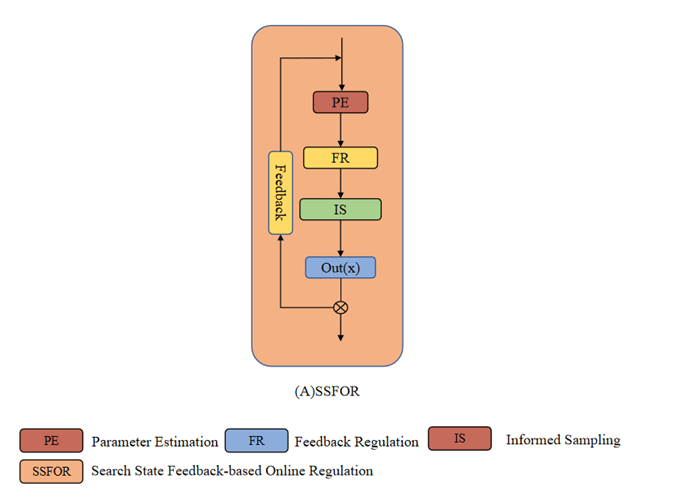
\includegraphics[width=0.8\textwidth]{fig3SSFOR.png} 
    \caption{Flow diagram of the Search State Feedback-Based Online Regulation (SSFOR) mechanism}
    \label{fig:ssfor_flowchart}
\end{figure}

To ensure the boundedness and reproducibility of the above adjustment process, this paper specifies the value range and initial states of the two parameters as follows: The super-ellipsoid expansion factor $\gamma$ is defined within the range $\gamma \in [1.0, 4.0]$, with a nominal value of $\gamma_0 = 1.5$. At algorithm initialization, $\gamma$ is set to 2.5 to ensure sufficient exploratory coverage during the early stage of the search. A larger $\gamma$ corresponds to a greater degree of super-ellipsoidal expansion, leading the algorithm to favor broader exploration. Conversely, a smaller $\gamma$ results in a more compact constrained sampling subset, causing the algorithm to shift toward intensified local convergence. The heuristic sampling probability $p$ is defined within the range $p \in [0.2, 0.95]$, with a nominal value of $p_0 = 0.8$. The initial value is set to the lower bound $p = 0.2$, so that before any feasible path is obtained, the algorithm relies entirely on global random sampling for initial exploration. A higher $p$ corresponds to a greater proportion of informed sampling, favoring refined local search; a lower $p$ increases the proportion of global random sampling, thereby maintaining search diversity. When the constraint is overly relaxed, a large number of nodes fall into inefficient regions; when it is overly restrictive, the effective sampling rate drops sharply in obstacle-dense environments. Under the closed-loop regulation of SSFOR, both parameters fluctuate within the aforementioned valid ranges, preventing unbounded expansion or excessive contraction of the constrained sampling subset, and ensuring that the constraint strength continuously matches the current stage of the search. The overall framework of SC-RRT, comprising the main search loop, SSFOR-based online regulation, and ADCS sampling, is illustrated in Figure~\ref{fig:fig4Overall_framework}.



\begin{figure}[h]
    \centering
    % 确保路径和文件名与左侧文件树完全一致
    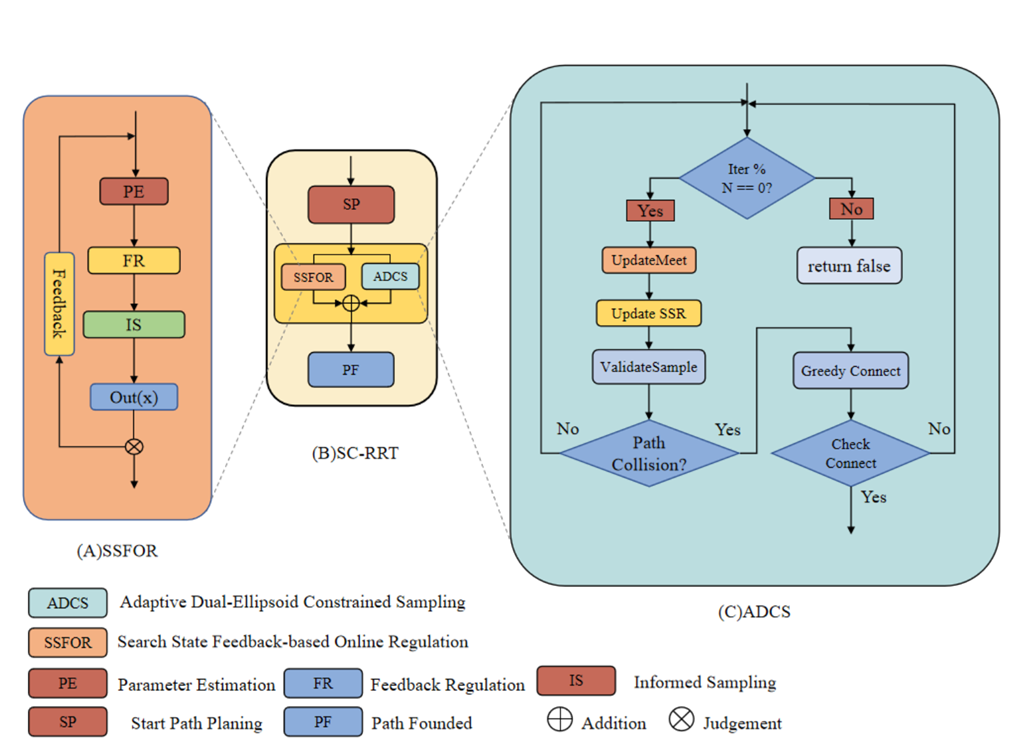
\includegraphics[width=0.8\textwidth]{fig4Overall_framework.png} 
    \caption{Overall framework of the SC-RRT algorithm. It consists of the main search loop, SSFOR-based online regulation, and ADCS sampling. Dashed arrows indicate the internal implementation of key modules}
    \label{fig:fig4Overall_framework}
\end{figure}



The sequential search process of SC-RRT in a representative 2D environment is depicted in Figure~\ref{fig:Path_planning_process_of_SC-RRT_in_a_2D_environment}, where the progressive convergence of the dual-super-ellipsoid constrained sampling regions can be observed.

\begin{figure}[h]
    \centering
    % 确保路径和文件名与左侧文件树完全一致
    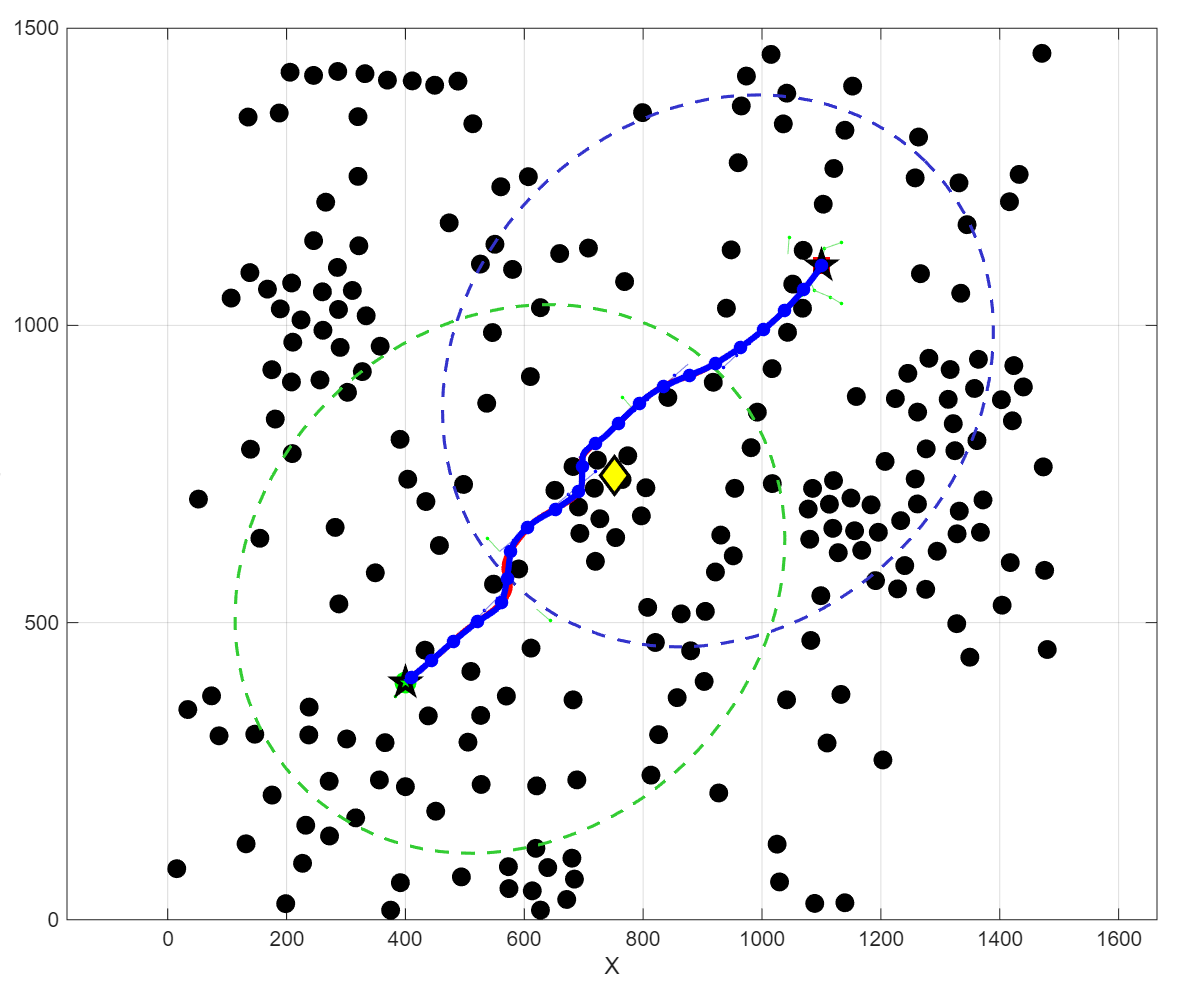
\includegraphics[width=0.8\textwidth]{fig5_path_planning_2d.png} 
    \caption{Path planning process of SC-RRT in a 2D environment.}
    \label{fig:Path_planning_process_of_SC-RRT_in_a_2D_environment}
\end{figure}

\section{Simulation}\label{sec4}

To systematically evaluate the performance of SC-RRT under consistent environmental scale and obstacle density, comparative simulation experiments were conducted in both two-dimensional and three-dimensional spaces. The results are shown in Figures~\ref{fig:62Dcompare_result} and~\ref{fig:fig73Dcompare_result}. The evaluation metrics include: Path Length, defined as the sum of the Euclidean distances between adjacent nodes along the path (mm); Convergence Time, defined as the time required for the algorithm to achieve path convergence (s); Node Count, defined as the total number of sampled nodes generated during the planning process; and The path efficiency $\eta$ is formally defined as:
\begin{equation}
\label{eq:path_efficiency}
\eta = \frac{\|\mathbf{x}_{\text{goal}} - \mathbf{x}_{\text{start}}\|}{L(\sigma)}
\end{equation}
where $L(\sigma) = \sum_{i=1}^{N-1} \|\mathbf{x}_{i+1} - \mathbf{x}_i\|$ is the total path length along the planned path $\sigma = \{\mathbf{x}_1, \mathbf{x}_2, \ldots, \mathbf{x}_N\}$, and $\|\mathbf{x}_{\text{goal}} - \mathbf{x}_{\text{start}}\|$ is the straight-line distance. Values of $\eta$ closer to 1.0 indicate near-optimal paths.




Based on previous studies in path planning, five representative algorithms---RRT, RRT-Connect, RRT*, Informed RRT*, and Dynamic-RRT---were selected for comparison with the proposed SC-RRT algorithm to validate its performance and stability. To ensure fairness in performance comparison among different path planning algorithms, all methods were evaluated under identical environmental spaces and obstacle configurations. Using the environment specified in Table~\ref{tab:env_config} as an example, each algorithm was executed 500 times, and performance metrics such as path length and convergence time were assessed.

\begin{table}[h]
\centering
\caption{Environment Configuration} % 建议加上标题
\label{tab:env_config}
%\begin{tabular}{|c|c|c|c|c|c|} % 根据实际列数调整，这里假设是6列
\begin{tabular}{cccccc}
\toprule 
dimension & Environment & Obstacles & Start & Goal & Max Iter \\
\midrule 
2 & $1500 \times 1500$ & 225 & $(75, 75)$ & $(1425, 1425)$ & 5000 \\
3 & $1500 \times 1500 \times 1500$ & 400 & $(75, 75, 75)$ & $(1425, 1425, 1425)$ & 8000 \\
\bottomrule 
\end{tabular}
\end{table}


\begin{figure}[h]
    \centering
    % 确保路径和文件名与左侧文件树完全一致
    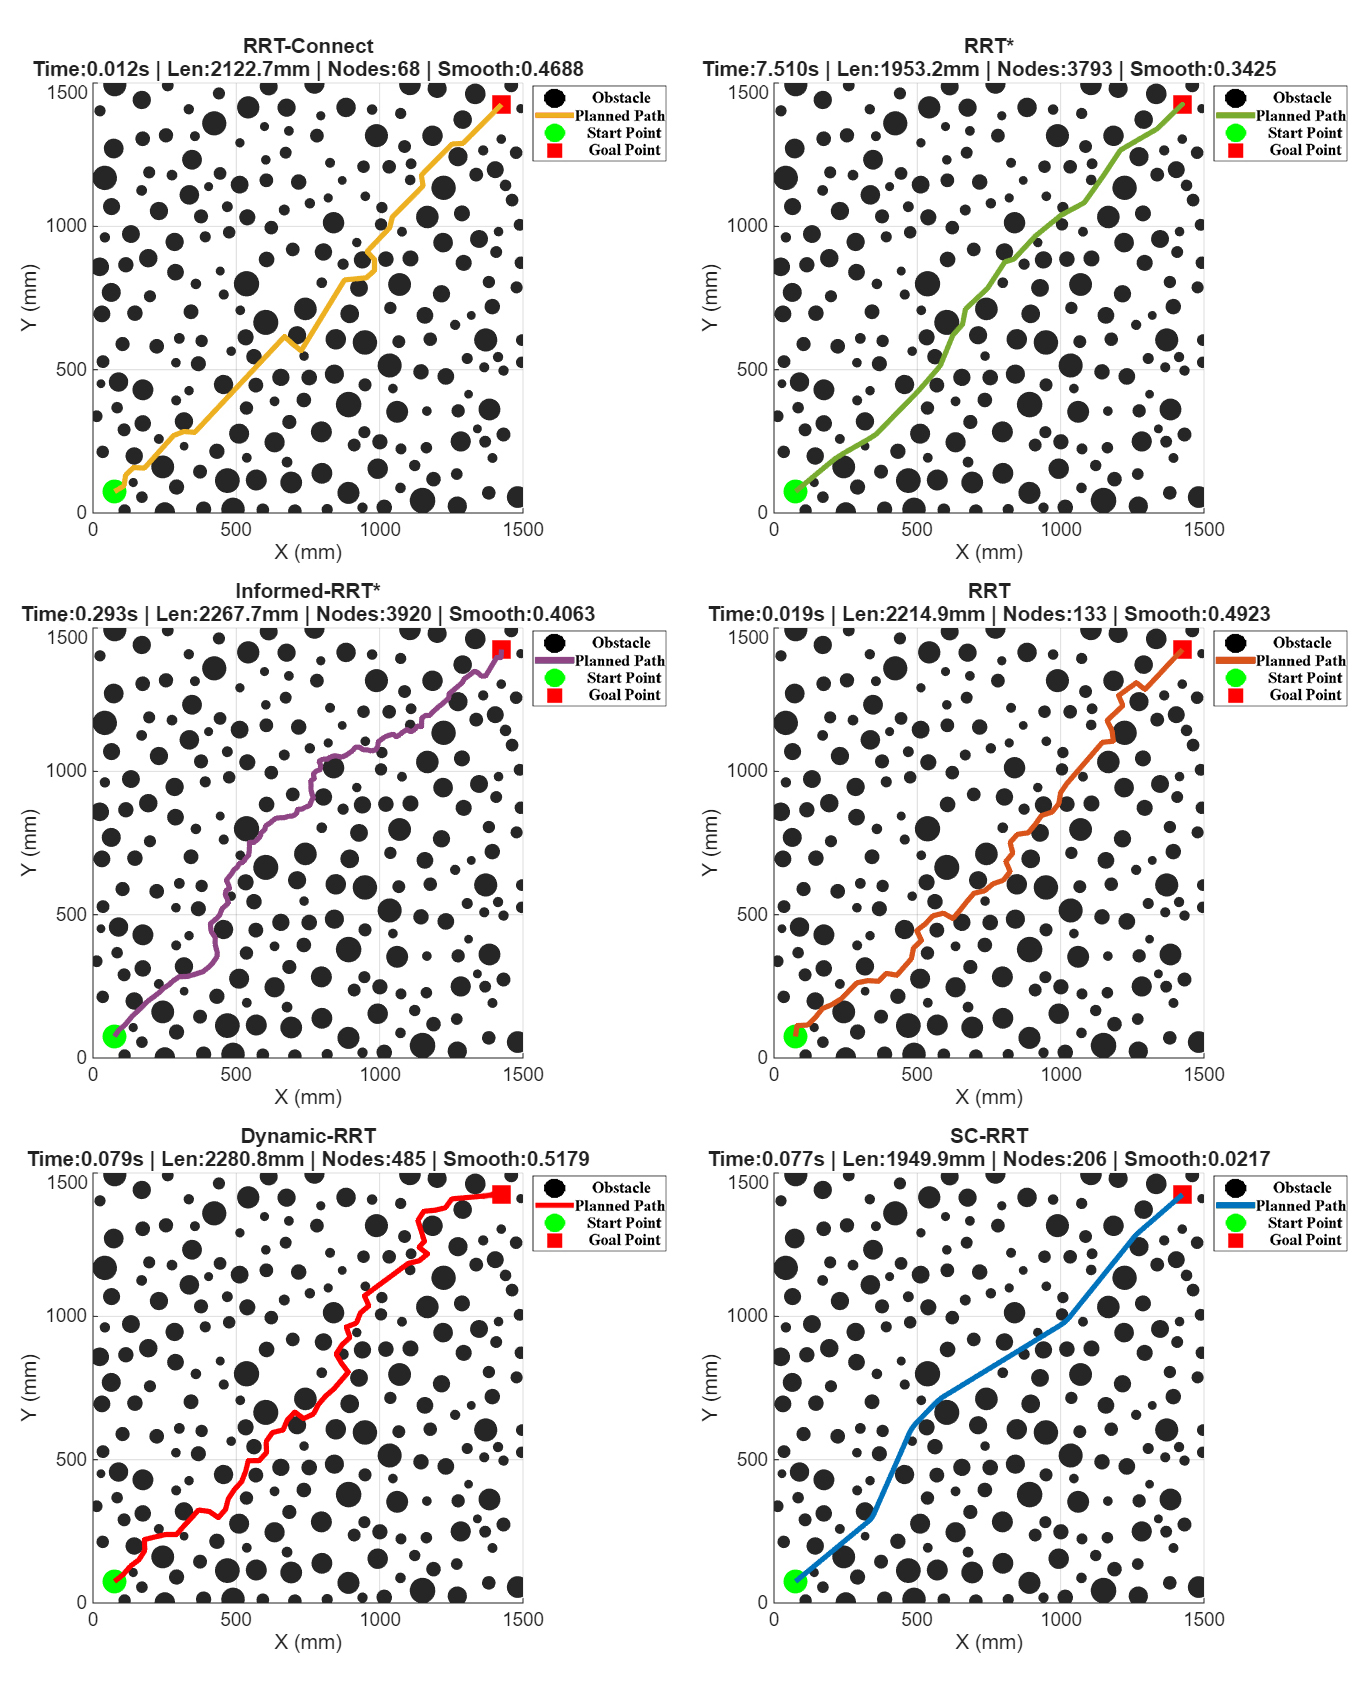
\includegraphics[width=0.8\textwidth]{fig62Dcompare_result.jpg} 
    \caption{Comparison Results of Different Path Planning Algorithms in Two-Dimensional Space.}
    \label{fig:62Dcompare_result}
\end{figure}


\begin{figure}[h]
    \centering
    % 确保路径和文件名与左侧文件树完全一致
    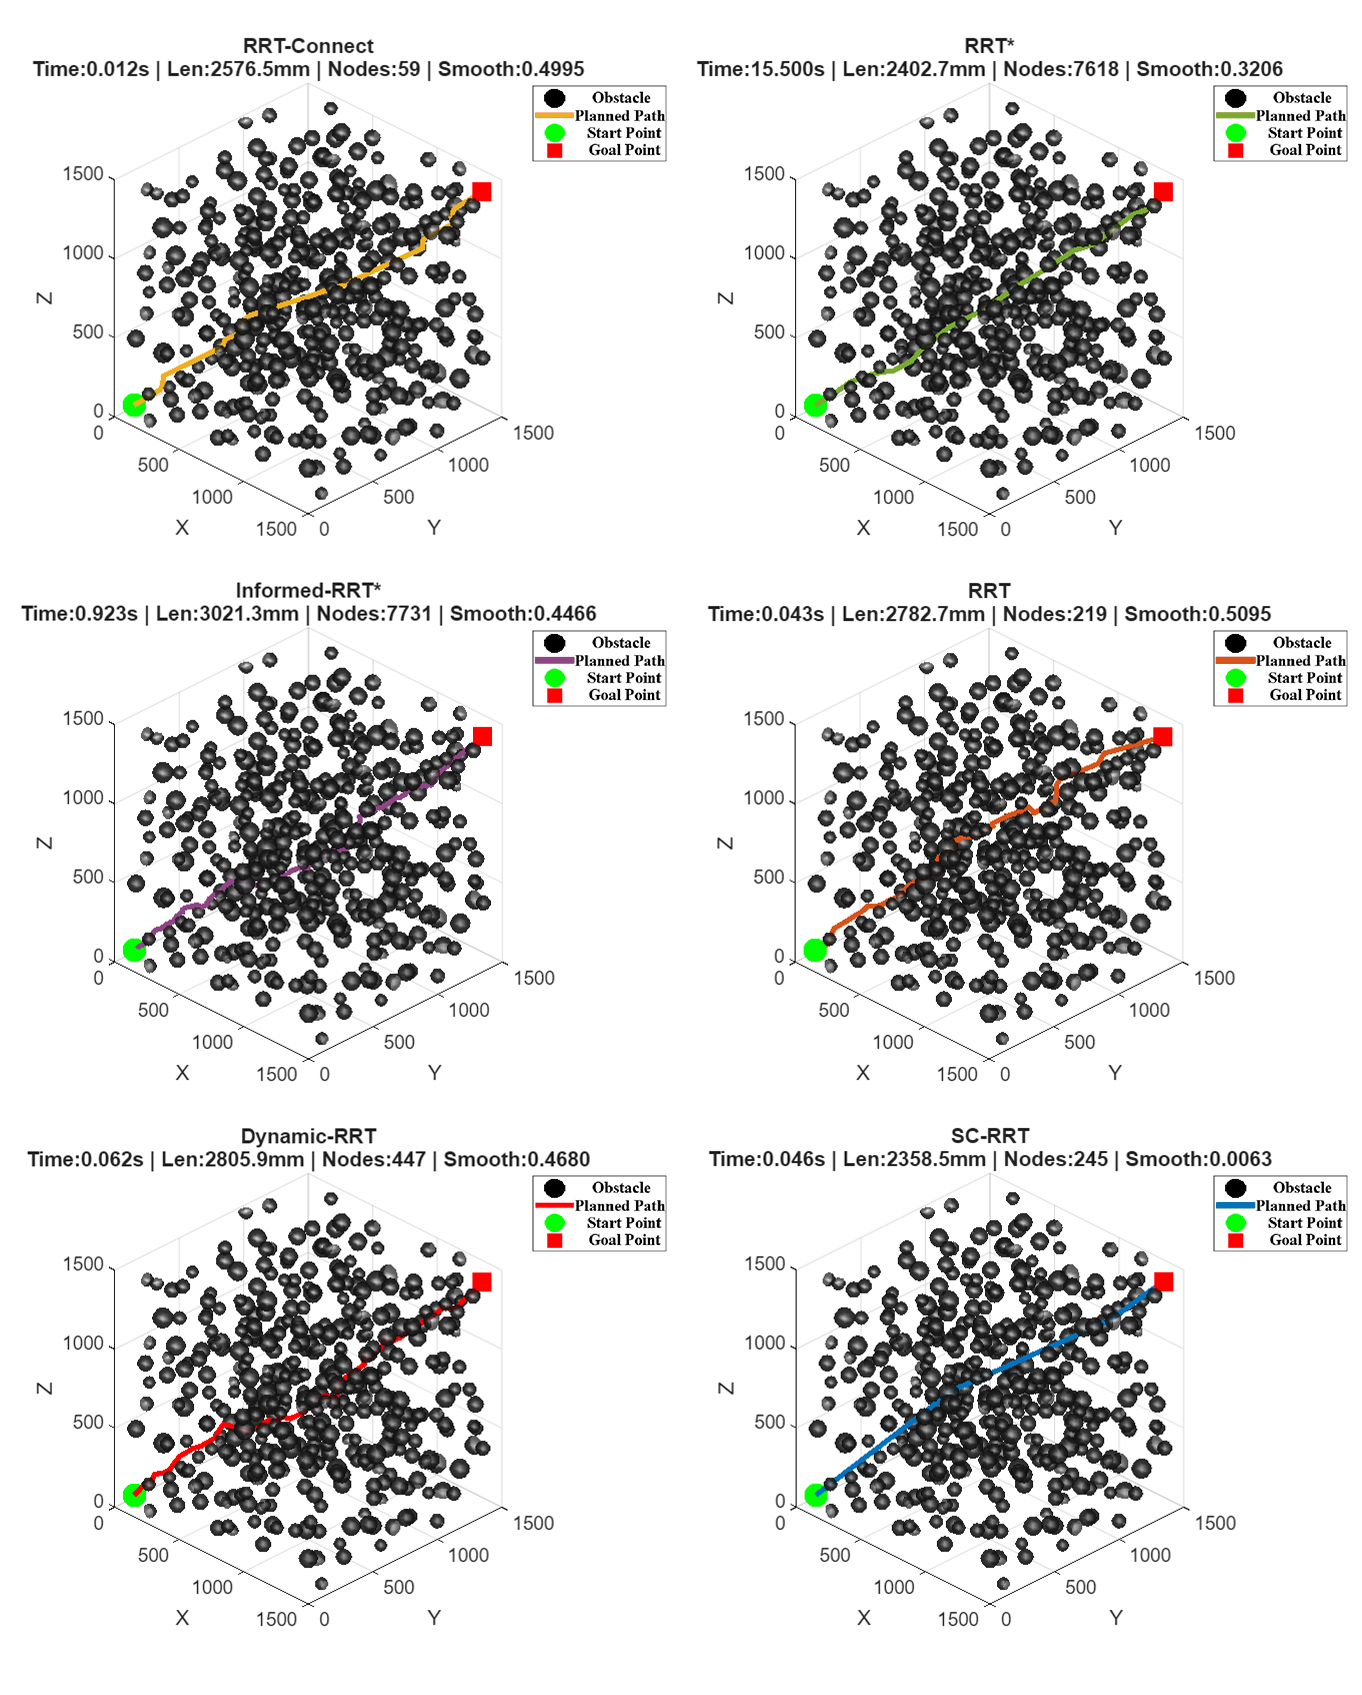
\includegraphics[width=0.8\textwidth]{fig73Dcompare_result.jpg} \caption{Comparison Results of Different Path Planning Algorithms in Three-Dimensional Space.}
    \label{fig:fig73Dcompare_result}
\end{figure}



Under typical scenarios with varying obstacle densities in both two-dimensional and three-dimensional spaces, a systematic comparison was conducted between SC-RRT and mainstream algorithms including RRT, RRT-Connect, RRT*, Informed RRT*, and Dynamic-RRT, under identical environmental configurations and computational budgets. The results are presented in Table~\ref{tab:algo_comparison}. Overall, the asymptotic optimality of Dynamic-RRT relies on sufficient computation time to be fully realized, which leads to notable limitations in scenarios with high real-time requirements. Although biasing the probability distribution of the random sample node $x_{rand}$ toward the goal direction yields some improvement in path length and efficiency metrics, the degree of enhancement remains limited. In contrast, leveraging the online adaptive regulation mechanism (SSFOR), SC-RRT significantly reduces convergence time and sampling scale while maintaining comparable path length, demonstrating superior overall real-time performance compared to Dynamic-RRT.

Regarding path quality, SC-RRT achieves an average path length of $2049.09$~mm. This represents a $10.5\%$ reduction compared to Dynamic-RRT and deviates by only $4.0\%$ from the asymptotically optimal RRT*, yet it incurs a fraction of the computational cost. With a path efficiency of $0.9553$, SC-RRT ranks third, trailing only the computationally intensive Informed RRT* and RRT*. Crucially, SC-RRT accomplishes this with a planning time that is just $16.2\%$ of Informed RRT*'s requirement. The marginal $1.40\%$ efficiency gap compared to RRT* highlights SC-RRT's ability to approach optimality without the associated time penalty. These metrics validate that the ADCS mechanism effectively concentrates sampling along near-straight corridors, minimizing detours while drastically accelerating convergence. Furthermore, the low standard deviation in path length ($\pm 57.53$~mm) confirms the algorithm's stability across diverse obstacle configurations.

In terms of computational efficiency, SC-RRT achieves an average convergence time of $0.0345$~s, with a node consumption of only $209.6$, demonstrating excellent real-time responsiveness. Although RRT* guarantees asymptotic optimality, it requires as many as $3846.6$ nodes and a convergence time of $0.1629$~s. In comparison, SC-RRT achieves nearly a $4.7$-fold speedup, highlighting its significant advantage in time-sensitive tasks.

In terms of path stability, SC-RRT exhibits a path length standard deviation of only $\pm 57.53$~mm, which is significantly lower than that of RRT ($\pm 126.25$~mm) and Dynamic-RRT ($\pm 136.02$~mm), demonstrating markedly superior consistency and reproducibility in planning results. In summary, SC-RRT achieves an optimal overall balance among path quality, computational efficiency, and planning stability. It maintains stable convergence and strong scalability across both two-dimensional and three-dimensional scenarios with varying obstacle densities, demonstrating robust generalization capability and substantial practical engineering value.

\begin{table}[h!]
\centering
\caption{Comparison of Path Planning Algorithms\label{tab:algo_comparison}}
\begin{tabular}{@{\extracolsep{\fill}}lcccc}
\hline
Algorithm & Path Length (mm) & Convergence Time (s) & Node Count & Path Efficiency\\
\hline
RRT & $2329.5500 \pm 126.2500$ & $0.0409 \pm 0.0305$ & $279.4000 \pm 175.5000$ & $0.8219 \pm 0.0429$\\
RRT-connect & $2143.2400 \pm 93.4900$ & $0.0108 \pm 0.0053$ & $69.3000 \pm 10.8000$ & $0.8924 \pm 0.0376$\\
RRT* & $1970.7200 \pm 19.9400$ & $0.1629 \pm 0.0843$ & $3846.6000 \pm 99.7000$ & $0.9689 \pm 0.0098$\\
Informed RRT* & $1938.4500 \pm 24.1300$ & $0.2134 \pm 0.0487$ & $3612.3000 \pm 108.6000$ & $0.9714 \pm 0.0076$\\
SC-RRT & $2049.0900 \pm 57.5300$ & $0.0345 \pm 0.0124$ & $209.6000 \pm 38.5000$ & $0.9553 \pm 0.0265$\\
Dynamic-RRT & $2288.1300 \pm 136.0200$ & $0.0414 \pm 0.0384$ & $281.3000 \pm 160.2000$ & $0.8372 \pm 0.0468$\\
\hline
\end{tabular}
\end{table}


\section{Conclusion}\label{sec5}

To address the issues of low effective sampling rates, slow convergence in obstacle-dense environments, and the sensitivity of informed subsets to cost estimation bias in sampling-based path planning algorithms, this paper proposes the SC-RRT algorithm. The algorithm comprises two tightly coupled core mechanisms.

First, Adaptive Asymmetric Dual-Super-Ellipsoidal Constrained Sampling (ADCS). A dynamically updated intermediate point, derived online from the bidirectional search state, is introduced to decompose the global planning task into two directional subproblems: ``start--intermediate'' and ``goal--intermediate.'' For each direction, a super-ellipsoidal informed subset with independently adjustable scale is constructed. Unlike Dynamic-RRT, which adopts a single symmetric ellipsoid with the start and goal as fixed focal points, the asymmetric dual-super-ellipsoid structure of ADCS enables directional compression and expansion according to the differing search progress on the two sides. While maintaining exploratory coverage, it significantly increases the sampling density along potentially feasible corridors, effectively mitigating the insufficient global guidance capability of single-direction frameworks highlighted in the introduction.

Second, the Search-State Feedback Online Regulation (SSFOR) mechanism. Using the current best path cost and its recent historical sequence as feedback signals, SSFOR dynamically outputs the super-ellipsoid expansion factor $\gamma$ and the informed sampling probability $p$, implementing closed-loop regulation over the volume of the informed subset and the sampling allocation ratio. When path improvement stagnates, the exploration range is automatically expanded; when improvement is efficient, the constraints are progressively tightened to enhance local convergence. In this way, the mechanism overcomes the sensitivity issues in traditional methods, where cost overestimation leads to an excessively large informed subset and cost underestimation results in premature contraction of the sampling region.

Under representative scenarios with varying obstacle densities in both two-dimensional and three-dimensional spaces, and under identical environmental configurations and computational budgets, SC-RRT---through the synergistic effect of ADCS's bidirectional asymmetric constraints and SSFOR's closed-loop regulation---demonstrates more consistent convergence behavior, fewer redundant expansions, and higher planning stability across different spatial dimensions and obstacle distributions. These results confirm that the integration of adaptive asymmetric dual-super-ellipsoidal constrained sampling with online constraint feedback regulation is an effective approach to enhancing the overall performance of sampling-based planning algorithms. It further provides a generalizable modeling framework for mitigating sensitivity to cost estimation bias in similar methods. SC-RRT inherits the probabilistic completeness of Informed RRT* and, within the asymptotic optimality framework, further accelerates convergence through bidirectional expansion and dynamic constraint regulation, thereby ensuring both theoretical soundness and engineering efficiency.

\backmatter
\bmhead{Acknowledgements}

The authors would like to thank the School of Mechanical Engineering, Shanghai Institute of Technology, for providing the computational resources.

\textbf{AI disclosure:} During the preparation of this manuscript, the authors used GitHub Copilot as a translation aid to translate the original Chinese draft into English. All AI-assisted output was carefully reviewed and edited by the authors, who take full responsibility for the accuracy, scientific integrity, and originality of the manuscript.

\section*{Declarations}

\textbf{Author contributions:} Xingyu Guo conceived the algorithm, conducted the simulation experiments, and drafted the manuscript. Yan Wu supervised the research and provided guidance on the overall manuscript. Muchun Fan and Feng Hong provided technical support during implementation. Hongyu Gao and Jianyu Zheng contributed to manuscript revision and provided valuable comments. All authors contributed to the conception and design of the study, and all authors read and approved the final manuscript.

\textbf{Funding:} This research received no specific grant from any funding agency, commercial, or not-for-profit sectors.

\textbf{Competing interests:} The authors declare no competing interests.

\textbf{Ethics approval:} Not applicable.

\textbf{Consent to participate:} Not applicable.

\textbf{Consent for publication:} All authors have approved the manuscript and agree to its submission for publication.

\textbf{Data availability:} The data that support the findings of this study are available from the corresponding author upon reasonable request.

\textbf{Code availability:} The code used in this study is available from the corresponding author upon reasonable request.



%%===========================================================================================%%
%% If you are submitting to one of the Nature Portfolio journals, using the eJP submission   %%
%% system, please include the references within the manuscript file itself. You may do this  %%
%% by copying the reference list from your .bbl file, paste it into the main manuscript .tex %%
%% file, and delete the associated \verb+\bibliography+ commands.                            %%
%%===========================================================================================%%

\bibliography{sn-bibliography}% common bib file
%% if required, the content of .bbl file can be included here once bbl is generated
%%\input sn-article.bbl

\end{document}
